\documentclass[aspectratio=169]{beamer}
\usepackage{xeCJK}
\usepackage{fontspec}
\usepackage{graphicx}
\usepackage{listings}
\usepackage{xcolor}
\usepackage{indentfirst}
\usepackage{tikz}
\usepackage{amssymb}
\usepackage{amsthm}
\usepackage{amsmath}
\usepackage{tabularx}
\usepackage{hyperref}
\usepackage{ulem}
\usepackage{version}
\usepackage{thmtools}
\usepackage{qtree}
\usepackage{algpseudocode}
\usepackage{mathtools}
\usepackage{multicol}
\usepackage{xcolor}
\usepackage{forest}
\usepackage{minted}

\XeTeXlinebreaklocale "zh"
\XeTeXlinebreakskip = 0pt plus 1pt

\setCJKmainfont{Noto Sans CJK TC}
\setmainfont{Noto Sans CJK TC}
\setmonofont{Ubuntu Mono}
\usetikzlibrary{arrows,decorations.markings,decorations.pathreplacing}

\lstset{
    basicstyle=\ttfamily\normalsize\color{black},
    commentstyle=\color{black!50},
    keywordstyle=\color{white!0!blue},
    stringstyle=\color{black!50!green},
    showspaces=false,
    showstringspaces=false,
    showtabs=false,
    tabsize=4,
    captionpos=b,
    breaklines=true,
    breakatwhitespace=false,
    escapeinside={\%*}{*)},
    morekeywords={*}
}
\forestset{
  default preamble = {
    for tree = {
      edge = {-},
      circle,
      minimum size=2.5em,
      inner sep=0pt,
      draw,
      math content,
      tier/.wrap pgfmath arg={tier #1}{level()},
      anchor=center,
      s sep = 2em
    }
  }
}

\title{Tree}
\author{上課補充 by PixelCat} % \\Credit by XXX
\date{}

\usetheme{sprout}

\setlength\parskip{12pt}
\makeatletter
\newcommand{\@minipagerestore}{\setlength{\parskip}{12pt}}
\makeatother

\hypersetup{colorlinks=true, linkcolor=SproutLinkColor, urlcolor=SproutURLColor}

\begin{document}

{\setbeamertemplate{background}
    {
\includegraphics[width=\paperwidth,height=\paperheight,keepaspectratio]{background_title.png}}
    \begin{frame}
        \titlepage
    \end{frame}
}

\section{課程影片}

\begin{frame}{課程影片}
    想一想,為什麼一般的binary tree不適合用陣列存呢?
\end{frame}

\begin{frame}{課程影片}
    善良的二元樹
    \begin{center}
        \scalebox{0.7}{
          \begin{forest}
            [1, fill=red!0!green!40!white
            [2, fill=red!0!green!40!white
              [4, fill=red!0!green!40!white
                [8, fill=red!0!green!40!white
                ]
                [9, fill=red!0!green!40!white
                ]
              ]
              [5, fill=red!0!green!40!white
                [10, fill=red!0!green!40!white
                ]
                [11, fill=red!0!green!40!white
                ]
              ]
            ]
            [3, fill=red!0!green!40!white
              [6, fill=red!0!green!40!white
                [12, fill=red!0!green!40!white
                ]
                [13, fill=red!0!green!40!white
                ]
              ]
              [7, fill=red!0!green!40!white
                [14, fill=red!0!green!40!white
                ]
                [15, fill=red!0!green!40!white
                ]
              ]
            ]
          ]  
          \end{forest}
        }
    \end{center}
\end{frame}

\begin{frame}{課程影片}
    邪惡的二元樹

    \begin{center}
        \scalebox{0.6}{
          \begin{forest}
            [1, fill=red!0!green!40!white
            [, phantom]
            [3, fill=red!0!green!40!white
              [, phantom]
              [7, fill=red!0!green!40!white
                [, phantom]
                [15, fill=red!0!green!40!white
                  [, phantom]
                  [, dashed, very thick, draw=blue
                    [, phantom]
                    [2 ^ n - 1, minimum size=4em, fill=red!0!green!40!white]
                  ]
                ]
              ]
            ]
          ]    
          \end{forest}
        }
    \end{center}
\end{frame}

\begin{frame}{課程影片}
    開一個長度是 $2 ^ n$ 的陣列,只用到其中 $n$ 個節點

    這怎麼可以\\
    乖乖用指標去
\end{frame}

\begin{frame}{課程影片}
    Q \& A?
\end{frame}


\section{二元搜尋樹}

\begin{frame}{二元搜尋樹}
    「二元搜尋樹」(Binary Search Tree,BST)\\
    是一種特別的樹,在資料結構中佔有重要的地位

    二元:一棵二元樹\\
    搜尋:你可以在樹上搜尋(???)
\end{frame}

\begin{frame}{二元搜尋樹}
    讓二元樹上每個節點都存一個值,而且對於每個節點:

    \begin{itemize}
        \item 他的左子樹內,所有節點的值都 $\leq$ 他的值
        \item 他的右子樹內,所有節點的值都 $\geq$ 他的值
        \item 他的左右子樹分別都是 BST
    \end{itemize}

    $\Rightarrow$ 二元搜尋樹的\textbf{中序遍歷}是從小到大排序好的
\end{frame}

\begin{frame}{二元搜尋樹}
    我們希望能一邊維護二元搜尋樹的性質,一邊支援:

    \begin{itemize}
        \item 查詢數字 $x$ 有沒有在樹上
        \item 加一個數字 $x$ 到樹上
        \item 從樹上刪掉一個數字 $x$
    \end{itemize}
\end{frame}

\begin{frame}{二元搜尋樹:範例}
    \begin{center}
        \scalebox{0.7}{
          \begin{forest}
            [9, fill=red!0!green!40!white
              [4, fill=red!0!green!40!white
                [2, fill=red!0!green!40!white
                ]
                [6, fill=red!0!green!40!white
                  [5, fill=red!0!green!40!white
                  ]
                  [7, fill=red!0!green!40!white
                  ]
                ]
              ]
              [19, fill=red!0!green!40!white
                [10, fill=red!0!green!40!white
                  [, phantom]
                  [16, fill=red!0!green!40!white
                  ]
                ]
                [20, fill=red!0!green!40!white]
              ]
            ]
          \end{forest}
        }
    \end{center}
\end{frame}

\begin{frame}{二元搜尋樹:查詢}
    % frame 1
    查詢 10 有沒有在樹上?

    \begin{center}
        \scalebox{0.7}{
          \begin{forest}
            [9, fill=blue!20!white
              [4, fill=red!0!green!40!white
                [2, fill=red!0!green!40!white
                ]
                [6, fill=red!0!green!40!white
                  [5, fill=red!0!green!40!white
                  ]
                  [7, fill=red!0!green!40!white
                  ]
                ]
              ]
              [19, fill=red!0!green!40!white
                [10, fill=red!0!green!40!white
                  [, phantom]
                  [16, fill=red!0!green!40!white
                  ]
                ]
                [20, fill=red!0!green!40!white]
              ]
            ]
          \end{forest}
        }
    \end{center}
\end{frame}

\begin{frame}{二元搜尋樹:查詢}
    % frame 2
    查詢 10 有沒有在樹上?

    \begin{center}
        \scalebox{0.7}{
          \begin{forest}
            [9, fill=red!100!green!40!white
              [4, fill=gray!40!white
                [2, fill=gray!40!white
                ]
                [6, fill=gray!40!white
                  [5, fill=gray!40!white
                  ]
                  [7, fill=gray!40!white
                  ]
                ]
              ]
              [19, fill=blue!20!white
                [10, fill=red!0!green!40!white
                  [, phantom]
                  [16, fill=red!0!green!40!white
                  ]
                ]
                [20, fill=red!0!green!40!white]
              ]
            ]
          \end{forest}
        }
    \end{center}
\end{frame}

\begin{frame}{二元搜尋樹:查詢}
    % frame 3
    查詢 10 有沒有在樹上?

    \begin{center}
        \scalebox{0.7}{
          \begin{forest}
            [9, fill=red!100!green!40!white
              [4, fill=gray!40!white
                [2, fill=gray!40!white
                ]
                [6, fill=gray!40!white
                  [5, fill=gray!40!white
                  ]
                  [7, fill=gray!40!white
                  ]
                ]
              ]
              [19, fill=red!100!green!40!white
                [10, fill=blue!20!white
                  [, phantom]
                  [16, fill=red!0!green!40!white
                  ]
                ]
                [20, fill=gray!40!white]
              ]
            ]
          \end{forest}
        }
    \end{center}
\end{frame}

\begin{frame}{二元搜尋樹:查詢}
    % frame 4
    好欸!找到了!

    \begin{center}
        \scalebox{0.7}{
          \begin{forest}
            [9
              [4
                [2
                ]
                [6
                  [5
                  ]
                  [7
                  ]
                ]
              ]
              [19
                [10, fill=red!0!green!40!white
                  [, phantom]
                  [16
                  ]
                ]
                [20]
              ]
            ]
          \end{forest}
        }
    \end{center}
\end{frame}

\begin{frame}{二元搜尋樹:查詢}
    % frame 1
    查詢 8 有沒有在樹上?

    \begin{center}
        \scalebox{0.7}{
          \begin{forest}
            [9, fill=blue!20!white
              [4, fill=red!0!green!40!white
                [2, fill=red!0!green!40!white
                ]
                [6, fill=red!0!green!40!white
                  [5, fill=red!0!green!40!white
                  ]
                  [7, fill=red!0!green!40!white
                  ]
                ]
              ]
              [19, fill=red!0!green!40!white
                [10, fill=red!0!green!40!white
                  [, phantom]
                  [16, fill=red!0!green!40!white
                  ]
                ]
                [20, fill=red!0!green!40!white]
              ]
            ]
          \end{forest}
        }
    \end{center}
\end{frame}

\begin{frame}{二元搜尋樹:查詢}
    % frame 2
    查詢 8 有沒有在樹上?

    \begin{center}
        \scalebox{0.7}{
          \begin{forest}
            [9, fill=red!100!green!40!white
              [4, fill=blue!20!white
                [2, fill=red!0!green!40!white
                ]
                [6, fill=red!0!green!40!white
                  [5, fill=red!0!green!40!white
                  ]
                  [7, fill=red!0!green!40!white
                  ]
                ]
              ]
              [19, fill=gray!40!white
                [10, fill=gray!40!white
                  [, phantom]
                  [16, fill=gray!40!white
                  ]
                ]
                [20, fill=gray!40!white]
              ]
            ]
          \end{forest}
        }
    \end{center}
\end{frame}

\begin{frame}{二元搜尋樹:查詢}
    % frame 3
    查詢 8 有沒有在樹上?

    \begin{center}
        \scalebox{0.7}{
          \begin{forest}
            [9, fill=red!100!green!40!white
              [4, fill=red!100!green!40!white
                [2, fill=gray!40!white
                ]
                [6, fill=blue!20!white
                  [5, fill=red!0!green!40!white
                  ]
                  [7, fill=red!0!green!40!white
                  ]
                ]
              ]
              [19, fill=gray!40!white
                [10, fill=gray!40!white
                  [, phantom]
                  [16, fill=gray!40!white
                  ]
                ]
                [20, fill=gray!40!white]
              ]
            ]
          \end{forest}
        }
    \end{center}
\end{frame}

\begin{frame}{二元搜尋樹:查詢}
    % frame 4
    查詢 8 有沒有在樹上?

    \begin{center}
        \scalebox{0.7}{
          \begin{forest}
            [9, fill=red!100!green!40!white
              [4, fill=red!100!green!40!white
                [2, fill=gray!40!white
                ]
                [6, fill=red!100!green!40!white
                  [5, fill=gray!40!white
                  ]
                  [7, fill=blue!20!white
                  ]
                ]
              ]
              [19, fill=gray!40!white
                [10, fill=gray!40!white
                  [, phantom]
                  [16, fill=gray!40!white
                  ]
                ]
                [20, fill=gray!40!white]
              ]
            ]
          \end{forest}
        }
    \end{center}
\end{frame}

\begin{frame}{二元搜尋樹:查詢}
    % frame 5
    找不到 QQ

    \begin{center}
        \scalebox{0.7}{
          \begin{forest}
            [9, fill=red!100!green!40!white
              [4, fill=red!100!green!40!white
                [2, fill=gray!40!white
                ]
                [6, fill=red!100!green!40!white
                  [5, fill=gray!40!white
                  ]
                  [7, fill=red!100!green!40!white
                  ]
                ]
              ]
              [19, fill=gray!40!white
                [10, fill=gray!40!white
                  [, phantom]
                  [16, fill=gray!40!white
                  ]
                ]
                [20, fill=gray!40!white]
              ]
            ]
          \end{forest}
        }
    \end{center}
\end{frame}

\begin{frame}{二元搜尋樹:查詢}
    回憶二元搜尋樹的性質「每個節點的左右子樹分別都是 BST」

    用遞迴的想法:

    \begin{itemize}
        \item 如果根節點就是要找的數字,那就是找到了
        \item 如果找到沒得找了還沒找到,那就是找不到
        \item 否則繼續找,拿根和目標數字比,決定往左還是往右
    \end{itemize}

    怎麼覺得有點像二分搜?

    \only<2> {
        再回憶性質「BST 的中序遍歷是從小到大排序好的」
    }
\end{frame}

\begin{frame}{二元搜尋樹:查詢}
    % frame 1
    查詢 10 有沒有在樹上?

    \begin{center}
        \scalebox{0.7}{
          \begin{forest}
            [9, fill=blue!20!white
              [4, fill=red!0!green!40!white
                [2, fill=red!0!green!40!white
                ]
                [6, fill=red!0!green!40!white
                  [5, fill=red!0!green!40!white
                  ]
                  [7, fill=red!0!green!40!white
                  ]
                ]
              ]
              [19, fill=red!0!green!40!white
                [10, fill=red!0!green!40!white
                  [, phantom]
                  [16, fill=red!0!green!40!white
                  ]
                ]
                [20, fill=red!0!green!40!white]
              ]
            ]
          \end{forest}
        }
    \end{center}

    \begin{figure}[h!]
        \begin{center}
            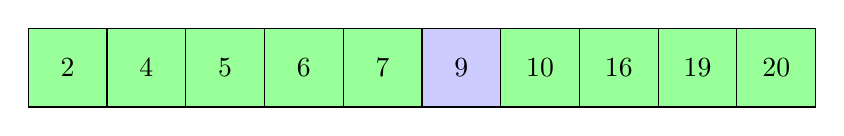
\begin{tikzpicture}
                \tikzset{x={(0.1cm, 0cm)}, y={(0cm, 0.1cm)}}
                \draw[fill=green!40!white] ( 0, 0) rectangle ( 10, 10) node[midway] {2};
                \draw[fill=green!40!white] (10, 0) rectangle ( 20, 10) node[midway] {4};
                \draw[fill=green!40!white] (20, 0) rectangle ( 30, 10) node[midway] {5};
                \draw[fill=green!40!white] (30, 0) rectangle ( 40, 10) node[midway] {6};
                \draw[fill=green!40!white] (40, 0) rectangle ( 50, 10) node[midway] {7};
                \draw[fill=blue!20!white] (50, 0) rectangle ( 60, 10) node[midway] {9};
                \draw[fill=green!40!white] (60, 0) rectangle ( 70, 10) node[midway] {10};
                \draw[fill=green!40!white] (70, 0) rectangle ( 80, 10) node[midway] {16};
                \draw[fill=green!40!white] (80, 0) rectangle ( 90, 10) node[midway] {19};
                \draw[fill=green!40!white] (90, 0) rectangle (100, 10) node[midway] {20};
            \end{tikzpicture}
        \end{center}
    \end{figure}
\end{frame}

\begin{frame}{二元搜尋樹:查詢}
    % frame 2
    查詢 10 有沒有在樹上?

    \begin{center}
        \scalebox{0.7}{
          \begin{forest}
            [9, fill=red!100!green!40!white
              [4, fill=gray!40!white
                [2, fill=gray!40!white
                ]
                [6, fill=gray!40!white
                  [5, fill=gray!40!white
                  ]
                  [7, fill=gray!40!white
                  ]
                ]
              ]
              [19, fill=blue!20!white
                [10, fill=red!0!green!40!white
                  [, phantom]
                  [16, fill=red!0!green!40!white
                  ]
                ]
                [20, fill=red!0!green!40!white]
              ]
            ]
          \end{forest}
        }
    \end{center}

    \begin{figure}[h!]
        \begin{center}
            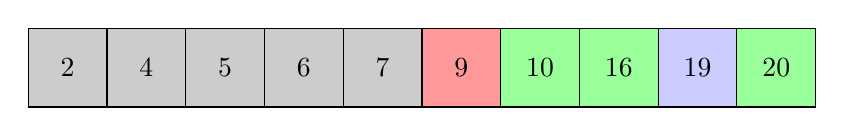
\begin{tikzpicture}
                \tikzset{x={(0.1cm, 0cm)}, y={(0cm, 0.1cm)}}
                \draw[fill=gray!40!white] ( 0, 0) rectangle ( 10, 10) node[midway] {2};
                \draw[fill=gray!40!white] (10, 0) rectangle ( 20, 10) node[midway] {4};
                \draw[fill=gray!40!white] (20, 0) rectangle ( 30, 10) node[midway] {5};
                \draw[fill=gray!40!white] (30, 0) rectangle ( 40, 10) node[midway] {6};
                \draw[fill=gray!40!white] (40, 0) rectangle ( 50, 10) node[midway] {7};
                \draw[fill=red!40!white] (50, 0) rectangle ( 60, 10) node[midway] {9};
                \draw[fill=green!40!white] (60, 0) rectangle ( 70, 10) node[midway] {10};
                \draw[fill=green!40!white] (70, 0) rectangle ( 80, 10) node[midway] {16};
                \draw[fill=blue!20!white] (80, 0) rectangle ( 90, 10) node[midway] {19};
                \draw[fill=green!40!white] (90, 0) rectangle (100, 10) node[midway] {20};
            \end{tikzpicture}
        \end{center}
    \end{figure}
\end{frame}

\begin{frame}{二元搜尋樹:查詢}
    % frame 3
    查詢 10 有沒有在樹上?

    \begin{center}
        \scalebox{0.7}{
          \begin{forest}
            [9, fill=red!100!green!40!white
              [4, fill=gray!40!white
                [2, fill=gray!40!white
                ]
                [6, fill=gray!40!white
                  [5, fill=gray!40!white
                  ]
                  [7, fill=gray!40!white
                  ]
                ]
              ]
              [19, fill=red!100!green!40!white
                [10, fill=blue!20!white
                  [, phantom]
                  [16, fill=red!0!green!40!white
                  ]
                ]
                [20, fill=gray!40!white]
              ]
            ]
          \end{forest}
        }
    \end{center}

    \begin{figure}[h!]
        \begin{center}
            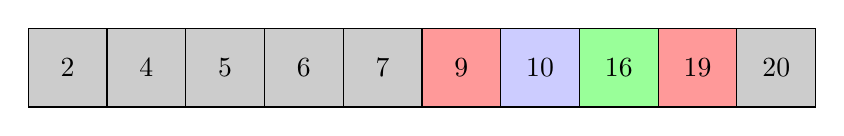
\begin{tikzpicture}
                \tikzset{x={(0.1cm, 0cm)}, y={(0cm, 0.1cm)}}
                \draw[fill=gray!40!white] ( 0, 0) rectangle ( 10, 10) node[midway] {2};
                \draw[fill=gray!40!white] (10, 0) rectangle ( 20, 10) node[midway] {4};
                \draw[fill=gray!40!white] (20, 0) rectangle ( 30, 10) node[midway] {5};
                \draw[fill=gray!40!white] (30, 0) rectangle ( 40, 10) node[midway] {6};
                \draw[fill=gray!40!white] (40, 0) rectangle ( 50, 10) node[midway] {7};
                \draw[fill=red!40!white] (50, 0) rectangle ( 60, 10) node[midway] {9};
                \draw[fill=blue!20!white] (60, 0) rectangle ( 70, 10) node[midway] {10};
                \draw[fill=green!40!white] (70, 0) rectangle ( 80, 10) node[midway] {16};
                \draw[fill=red!40!white] (80, 0) rectangle ( 90, 10) node[midway] {19};
                \draw[fill=gray!40!white] (90, 0) rectangle (100, 10) node[midway] {20};
            \end{tikzpicture}
        \end{center}
    \end{figure}
\end{frame}

\begin{frame}{二元搜尋樹:查詢}
    % frame 4
    好欸!找到了!

    \begin{center}
        \scalebox{0.7}{
          \begin{forest}
            [9
              [4
                [2
                ]
                [6
                  [5
                  ]
                  [7
                  ]
                ]
              ]
              [19
                [10, fill=red!0!green!40!white
                  [, phantom]
                  [16
                  ]
                ]
                [20]
              ]
            ]
          \end{forest}
        }
    \end{center}

    \begin{figure}[h!]
        \begin{center}
            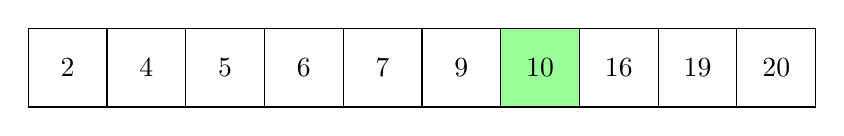
\begin{tikzpicture}
                \tikzset{x={(0.1cm, 0cm)}, y={(0cm, 0.1cm)}}
                \draw[] ( 0, 0) rectangle ( 10, 10) node[midway] {2};
                \draw[] (10, 0) rectangle ( 20, 10) node[midway] {4};
                \draw[] (20, 0) rectangle ( 30, 10) node[midway] {5};
                \draw[] (30, 0) rectangle ( 40, 10) node[midway] {6};
                \draw[] (40, 0) rectangle ( 50, 10) node[midway] {7};
                \draw[] (50, 0) rectangle ( 60, 10) node[midway] {9};
                \draw[fill=green!40!white] (60, 0) rectangle ( 70, 10) node[midway] {10};
                \draw[] (70, 0) rectangle ( 80, 10) node[midway] {16};
                \draw[] (80, 0) rectangle ( 90, 10) node[midway] {19};
                \draw[] (90, 0) rectangle (100, 10) node[midway] {20};
            \end{tikzpicture}
        \end{center}
    \end{figure}
\end{frame}

\begin{frame}{二元搜尋樹:插入}
    一般陣列不能隨便插入,但二元搜尋樹可以

    對於一個新節點,我們讓他當葉子,找個地方接在最下面
\end{frame}

\begin{frame}{二元搜尋樹:插入}
插入節點 10

\begin{center}
  \scalebox{0.7}{
    \begin{forest}
      [9, fill=blue!20!white
        [4, fill=none
          [2, fill=none
          ]
          [6, fill=none
            [5, fill=none
            ]
            [7, fill=none
            ]
          ]
        ]
        [19, fill=none
          [10, fill=none
            [, phantom]
            [16, fill=none
            ]
          ]
          [20, fill=none
          ]
        ]
      ]
    \end{forest}
  }
\end{center}
\end{frame}

\begin{frame}{二元搜尋樹:插入}
插入節點 10

\begin{center}
  \scalebox{0.7}{
    \begin{forest}
      [9, fill=red!40!white
        [4, fill=gray!40!white
          [2, fill=gray!40!white
          ]
          [6, fill=gray!40!white
            [5, fill=gray!40!white
            ]
            [7, fill=gray!40!white
            ]
          ]
        ]
        [19, fill=blue!20!white
          [10, fill=none
            [, phantom]
            [16, fill=none
            ]
          ]
          [20, fill=none
          ]
        ]
      ]
    \end{forest}
  }
\end{center}
\end{frame}

\begin{frame}{二元搜尋樹:插入}
插入節點 10

\begin{center}
  \scalebox{0.7}{
    \begin{forest}
      [9, fill=red!40!white
        [4, fill=gray!40!white
          [2, fill=gray!40!white
          ]
          [6, fill=gray!40!white
            [5, fill=gray!40!white
            ]
            [7, fill=gray!40!white
            ]
          ]
        ]
        [19, fill=red!40!white
          [10, fill=blue!20!white
            [, phantom]
            [16, fill=none
            ]
          ]
          [20, fill=gray!40!white
          ]
        ]
      ]
    \end{forest}
  }
\end{center}
\end{frame}

\begin{frame}{二元搜尋樹:插入}
插入節點 10

\begin{center}
  \scalebox{0.7}{
    \begin{forest}
      [9, fill=red!40!white
        [4, fill=gray!40!white
          [2, fill=gray!40!white
          ]
          [6, fill=gray!40!white
            [5, fill=gray!40!white
            ]
            [7, fill=gray!40!white
            ]
          ]
        ]
        [19, fill=red!40!white
          [10, fill=red!40!white
            [10, fill=green!40!white
            ]
            [16, fill=gray!40!white
            ]
          ]
          [20, fill=gray!40!white
          ]
        ]
      ]
    \end{forest}
  }
\end{center}
\end{frame}

\begin{frame}{二元搜尋樹:刪除}
    一般陣列不能隨便刪除,但二元搜尋樹可以

    第一階段:找到要刪掉的節點在哪\\
    第二階段:刪掉他\\
    第三階段:找個人把洞補起來
\end{frame}

\begin{frame}{二元搜尋樹:插入}
刪除節點 4\\
第一階段:找到要刪掉的節點

\begin{center}
  \scalebox{0.7}{
    \begin{forest}
      [9, fill=none
        [4, fill=blue!20!white
          [2, fill=none
          ]
          [6, fill=none
            [5, fill=none
            ]
            [7, fill=none
            ]
          ]
        ]
        [19, fill=none
          [10, fill=none
            [, phantom]
            [16, fill=none
            ]
          ]
          [20, fill=none
          ]
        ]
      ]
    \end{forest}
  }
\end{center}
\end{frame}

\begin{frame}{二元搜尋樹:插入}
刪除節點 4\\
第二階段:刪掉他

\begin{center}
  \scalebox{0.7}{
    \begin{forest}
      [9, fill=none
        [, fill=none, line width=2pt, draw=red
          [2, fill=none
          ]
          [6, fill=none
            [5, fill=none
            ]
            [7, fill=none
            ]
          ]
        ]
        [19, fill=none
          [10, fill=none
            [, phantom]
            [16, fill=none
            ]
          ]
          [20, fill=none
          ]
        ]
      ]
    \end{forest}
  }
\end{center}

樹上出現一個「洞」
\end{frame}

\begin{frame}{二元搜尋樹:插入}
刪除節點 4\\
第三階段:找個人把洞補起來

\begin{center}
  \scalebox{0.7}{
    \begin{forest}
      [9, fill=none
        [, fill=none, line width=2pt, draw=red
          [2, fill=green!40!white
          ]
          [6, fill=none
            [5, fill=green!40!white
            ]
            [7, fill=none
            ]
          ]
        ]
        [19, fill=none
          [10, fill=none
            [, phantom]
            [16, fill=none
            ]
          ]
          [20, fill=none
          ]
        ]
      ]
    \end{forest}
  }
\end{center}

用「左子樹最左邊的節點」或「右子樹最左邊的節點」來補\\
沒子樹怎麼辦?葉子可以直接拔掉
\end{frame}

\begin{frame}{二元搜尋樹:插入}
    刪除節點 4

    \begin{center}
        \scalebox{0.7}{
          \begin{forest}
            [9, fill=none
              [5, fill=green!40!white
                [2, fill=none
                ]
                [6, fill=none
                  [, phantom]
                  [7, fill=none
                  ]
                ]
              ]
              [19, fill=none
                [10, fill=none
                  [, phantom]
                  [16, fill=none
                  ]
                ]
                [20, fill=none
                ]
              ]
            ]
          \end{forest}
        }
    \end{center}      
\end{frame}

\begin{frame}{二元搜尋樹:時間複雜度}
    搜尋、插入、刪除,都是每回合需要 $O(1)$ 時間,從根出發每做完一個回合都往更深的節點走

    時間複雜度都是 $O(\text{樹的深度})$

    \only<2>{二元搜尋樹能有多深?}
\end{frame}

\begin{frame}{二元搜尋樹:時間複雜度}
    善良的二元樹
    \begin{center}
        \scalebox{0.7}{
          \begin{forest}
            [1, fill=red!0!green!40!white
            [2, fill=red!0!green!40!white
              [4, fill=red!0!green!40!white
                [8, fill=red!0!green!40!white
                ]
                [9, fill=red!0!green!40!white
                ]
              ]
              [5, fill=red!0!green!40!white
                [10, fill=red!0!green!40!white
                ]
                [11, fill=red!0!green!40!white
                ]
              ]
            ]
            [3, fill=red!0!green!40!white
              [6, fill=red!0!green!40!white
                [12, fill=red!0!green!40!white
                ]
                [13, fill=red!0!green!40!white
                ]
              ]
              [7, fill=red!0!green!40!white
                [14, fill=red!0!green!40!white
                ]
                [15, fill=red!0!green!40!white
                ]
              ]
            ]
          ]  
          \end{forest}
        }
    \end{center}
\end{frame}

\begin{frame}{二元搜尋樹:時間複雜度}
    邪惡的二元樹

    \begin{center}
        \scalebox{0.6}{
          \begin{forest}
            [1, fill=red!0!green!40!white
            [, phantom]
            [3, fill=red!0!green!40!white
              [, phantom]
              [7, fill=red!0!green!40!white
                [, phantom]
                [15, fill=red!0!green!40!white
                  [, phantom]
                  [, dashed, very thick, draw=blue
                    [, phantom]
                    [2 ^ n - 1, minimum size=4em, fill=red!0!green!40!white]
                  ]
                ]
              ]
            ]
          ]    
          \end{forest}
        }
    \end{center}
\end{frame}

\begin{frame}{二元搜尋樹:時間複雜度}
    二元搜尋樹能有多深?
    
    理想上「平衡的」二元搜尋樹深度應該要只有 $O(\log N)$\\
    但是最差甚至會到 $O(N)$

    \only<2>{所以對於一般二元搜尋樹,搜尋、插入、刪除的複雜度都是最糟 $O(N)$}
\end{frame}

\begin{frame}{二元搜尋樹:時間複雜度}
    要怎麼禁止二元搜尋樹不平衡?

    \begin{itemize}
        \item B-tree
        \item AVL tree
        \item 紅黑樹
        \item Treap
        \item Splay
        \item ...etc.
    \end{itemize}

    都好難好難,今天不會教
\end{frame}


\section{指標與偽指標}

\begin{frame}{指標}
    以二元樹為例,我們需要存左右子節點的指標

    但是好像很多人討厭指標?
\end{frame}

\begin{frame}[fragile]{指標}
    \begin{minted}{cpp}
        struct Node {
            Node *l, *r;
            int data;
        };

        Node *root = new Node();
        cout << root->data << "\n";
        delete root;  // 不釋放記憶體會怎樣嗎?
    \end{minted}
\end{frame}

\begin{frame}[fragile]{偽指標}
    \begin{minted}{cpp}
        struct Node {
            int l, r;
            int data;
        };
        Node nodes[MAX_NODE];  // 0 號節點代表空指標
        int _nodes_count = 0;

        int root = ++_nodes_count;
        cout << nodes[root].data << "\n";
        // 不需要釋放記憶體
    \end{minted}
\end{frame}

\begin{frame}{指標 v.s. 偽指標}
    \begin{columns}[totalwidth=\textwidth]
        \begin{column}{0.5\textwidth}
            指標:
        
            \begin{itemize}
                \item 用\textbf{指標} 代表每個節點
                \item 程式碼美觀
                \item 不用事先決定要開多少節點
            \end{itemize}
        \end{column}
        \begin{column}{0.5\textwidth}
            偽指標:

            \begin{itemize}
                \item 用\textbf{編號} 代表每個節點
                \item 方便 debug、輸出節點長相
                \item (一定程度上)避免戳到空指標原地 RE
                \item 不需要動態分配記憶體,比 new/delete 快一點點
                \item 整數比指標不佔空間
            \end{itemize}
        \end{column}
    \end{columns}
\end{frame}

\begin{frame}[fragile]{聰明的指標}
    \begin{minted}{cpp}
        struct Node {
            std::shared_ptr<Node> l, r;
            int data;
        };

        std::shared_ptr<Node> root = make_shared<Node>();
        cout << root->data << "\n";
        // 不需要特別釋放記憶體!
    \end{minted}
\end{frame}

\begin{frame}{聰明的指標}
    \begin{itemize}
        \item C++ smart pointers (C++ 11 或更新版本)
        \item 用法跟一般指標完全相同
        \item 自動回收記憶體避免 memory leak,輕鬆讓 \mintinline{bash}|-fsanitize=address| 閉嘴
        \item 競程幾乎(完全)沒人用
    \end{itemize}
\end{frame}

\end{document}
